\documentclass[conference, a4paper, 11pt]{IEEEtran}
\IEEEoverridecommandlockouts

\usepackage{amsmath,amssymb,amsfonts}
\usepackage{algorithmic}
\usepackage{graphicx}
\usepackage{textcomp}
\usepackage{xcolor}
\usepackage{hyperref}
\usepackage{subcaption}
\usepackage{caption}
\usepackage[
    backend = biber,
    language = auto,
    style = numeric,
    sorting = none,
    block = space,
    hyperref = true,
    bibencoding = auto,
    giveninits = true,
    doi=false,
    isbn=false,
    alldates=short
]{biblatex}
\addbibresource{literature.bib}
\usepackage{tabularx} % in the preamble
\usepackage{nameref}

\captionsetup{justification=centering,margin=0.5cm}

\def\BibTeX{{\rm B\kern-.05em{\sc i\kern-.025em b}\kern-.08em
    T\kern-.1667em\lower.7ex\hbox{E}\kern-.125emX}}
\begin{document}

\title{3DCV - Critical Driving Scenarios\\
{\small Generate critical driving scenarios in CARLA simulator and evaluate imitation learning possibilities}
}

\author{
    \IEEEauthorblockN{Christopher Klammt}
    \and
    \IEEEauthorblockN{Tobias Richstein}
    \and
    \IEEEauthorblockN{Julian Seibel}
    \and
    \IEEEauthorblockN{Karl Thyssen}
}

\maketitle

\begin{abstract}
	In this project report, we present an approach for generating new scenarios to support autonomous driving tasks in critical situations using the CARLA simulator along with its Scenario-Runner. Our approach consists of generating new XML-based OpenSCENARIO files which can be interpreted by the Scenario-Runner. Based on already present basic Scenarios, we apply a variety  of changes to attributes which are crucial for different sensors of an autonomous car. We considered external factors like weather, road conditions, time of day, color and models of cars, cyclists and pedestrians. In a second step, we transform the scenarios to different places in the same town and to different towns. To ensure the newly generated scenarios are valid, we consider different sanity checks as well as a specific verification to avoid duplicating scenarios.
	Additionally, we evaluated the possibilities for generating training data using the CARLA simulator as well as training an autonomous agent via imitation learning. For the training data the camera images can be obtained easily, whereas the expert input caused some issues. Both can - to a certain extent - be generated via a slightly modified script of the Scenario-Runner.

\end{abstract}

\begin{IEEEkeywords}
CARLA simulator, Scenario generation, Critical driving scenarios, Imitation learning, Autonomous driving
\end{IEEEkeywords}

\section{Introduction}
Autonomous driving vehicles are not just an idea for the more distant future, but rather a very current topic.
Not only Tesla, the company that dominates the news in this regard, is showing how far autonomous driving has come in the last years.
One crucial issue still lies in providing a stable and safe behavior in critical situations, especially those in which traffic participants behave unexpectedly. 
The problem is that to robustly learn the appropriate behavior for these specific critical scenarios and to generalize using supervised learning a large amount of training data is needed.

In order to tackle this problem, our paper describes the development of a generator for such critical driving scenarios in the CARLA simulator.
These critical driving scenarios are mainly inspired by the report \citetitle{NHTSA:PreCrashScenarios} \cite{NHTSA:PreCrashScenarios} for the National Highway Traffic Safety Administration in the United States.
These contain scenarios such as avoiding an obstacle, lane changing with oncoming traffic or crossing traffic running a red light at an intersection (as shown in \autoref{fig:scenario-run_red_light}).

\begin{figure}[ht]
    \centering
    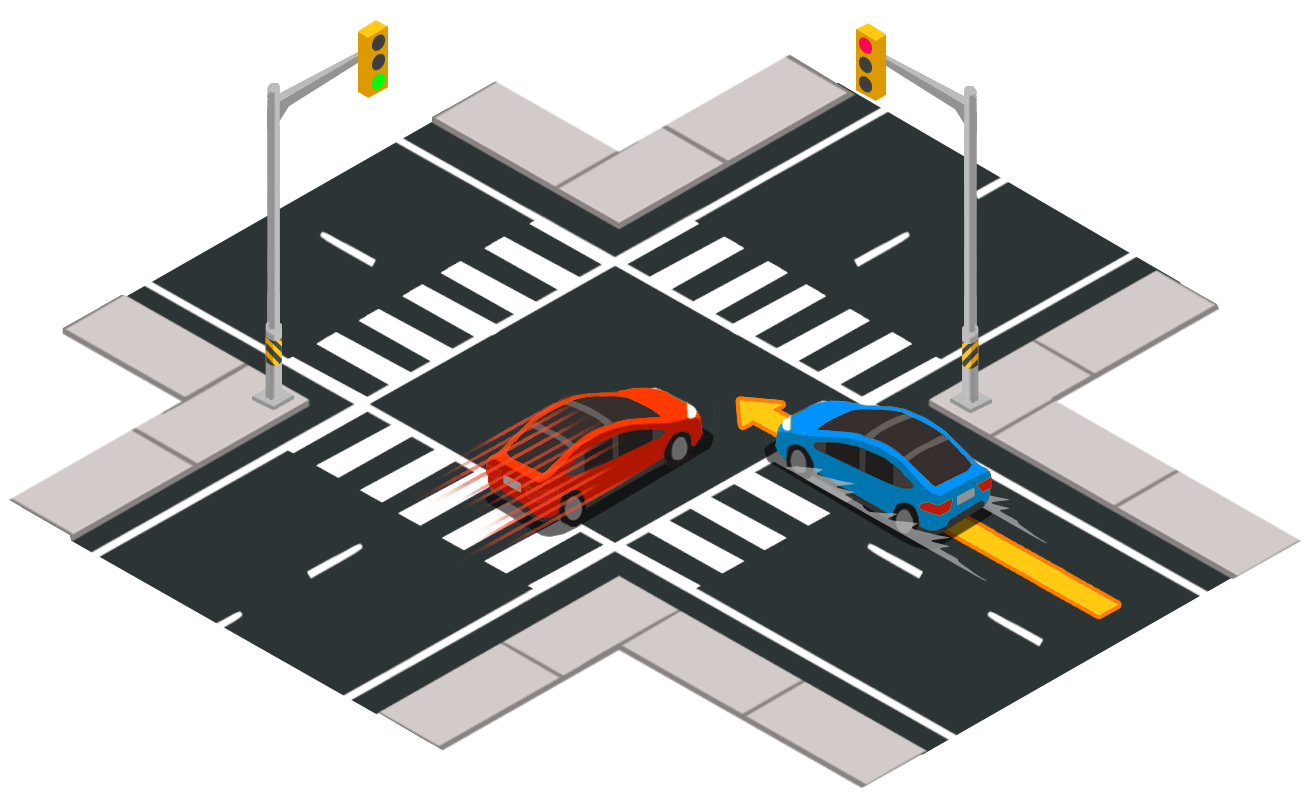
\includegraphics[width=0.7\linewidth]{figures/scenario-run_red_light.png}
    \caption{NHTSA scenario: Crossing traffic running a red light at an intersection \cite{CARLAChallenge:Scenarios}}
    \label{fig:scenario-run_red_light}
\end{figure}

Furthermore, after generating these different critical driving scenarios we utilize them to evaluate the possibilities of learning a robust autonomous agent.
To do so we focus on some prior papers using imitation learning, in which an expert demonstrates the desired behavior in each critical situation and is then adopted by the model.

\section{Related Work}

\subsection{CARLA}
As presented by \citeauthor{Dosovitskiy17:CARLA}, CARLA is an open-source urban driving simulator for autonomous driving research \cite{Dosovitskiy17:CARLA}.
It enables handling different use cases within the general problem of driving, such as learning driving policies or training perception algorithms.
To control the simulation, e.g. changing weather, adding cars or pedestrians, an API is available in Python and C++.
CARLA consists of the simulator responsible for rendering etc. as well as multiple components, for example a traffic manager controlling the vehicles or a component handling the sensors.

\subsection{Critical driving scenarios}

Another component that works in unison with the CARLA simulator is the Scenario-Runner \cite{CARLA:ScenarioRunner}.
This is a module that makes it possible to define various traffic scenarios and execute them in the CARLA simulator.
These scenarios can be defined using Python or the OpenSCENARIO \cite{OpenScenario} standard.
The Scenario-Runner already contains some predefined scenarios which are based on the critical driving scenarios as described in \citetitle{NHTSA:PreCrashScenarios} \cite{NHTSA:PreCrashScenarios}.

\subsection{Generating data in simulators}

In order to generate data it first is necessary to identify parameters that are to be adjusted and that should vary across the different entities.
The data generation can then be approached in different ways.
One possibility is to use a random statistical distribution of these parameters. 

Another way to go about data generation is to use learning-based methods to adjust the parameters of the simulator.
Such an approach was chosen by \citeauthor{DBLP:LearningToSimulate} and published in \citetitle{DBLP:LearningToSimulate} \cite{DBLP:LearningToSimulate}.
They proposed a reinforcement learning-based method to adjust the parameters of the synthesized data to maximize the accuracy of a model trained on that data.
A quite similar approach was chosen by \citeauthor{DBLP:Meta-Sim} \cite{DBLP:Meta-Sim} called Meta-Sim, which learns a generative model of synthetic scenes and modifies the attributes using a neural network.

\subsection{Learning an autonomous agent}

To learn a model based on labeled data some form of supervised learning is generally applied.
\citeauthor{Chen:LearningByCheating} propose a method called \citetitle{Chen:LearningByCheating} \cite{Chen:LearningByCheating}.
This is a two-stage method, in which first an agent is trained using privileged information.
In the second stage, the privileged agent acts as a teacher that trains a purely vision-based agent.

Another approach is \citetitle{Toromanoff_2020_CVPR} \cite{Toromanoff_2020_CVPR}. Here reinforcement learning is utilized to learn an optimal behavior policy based on a reward-function, effectively punishing wrong behavior such as leaving the track or running over pedestrians.

To train and manage the training of imitation learning networks jointly with evaluations on the CARLA simulator \citetitle{felipecode:coiltraine} \cite{felipecode:coiltraine} can be used.

\section{Method}

\subsection{Generating new scenarios through Scenario-Runner}
In general, we identified the two possible ways to create new scenarios that are supported by the Scenario-Runner.
The first option consists of using the Python based API of the Scenario-Runner library to define the dynamic behavior of every actor in combination with an \texttt{XML}-based configuration file, which can be used to initialize different parameters for a predefined Python based scenario.

The second option is to utilize OpenSCENARIO-based configuration files. OpenSCENARIO is an \texttt{XML}-based file standard for describing dynamic contents in driving simulation applications \cite{OpenScenario}. These configuration files differ from the previous approach mainly in one aspect. For defining OpenSCENARIO based scenarios, there is no need to create the Python-based scenario description. Therefore OpenSCENARIO can be used to generate all configurations for executing a scenario through the Scenario-Runner library combined at once. 

Both introduced options come with advantages and disadvantages. For our decision process, we identified different criteria which we would expect to be fulfilled for the approach we want to work with. 
The first criteria is \textit{generalization}. We would expect that the approach can be well generalized in terms of  extracting an abstract process which can be applied to all the different formats a new scenario could possibly have.
The second criteria is \textit{the number of directly accessible and adjustable parameters}. Since we aim to provide a scenario generation process which is capable of generating as many scenarios as possible, we want to achieve a high number of adjustable parameters for providing a large combinatoric basis. Moreover, the number of directly accessible parameters is crucial for ensuring a simple and well structured replacing process.
The third and last criteria we considered is \textit{simplicity} of the overall concept. Reducing the complexity and  following the KISS (Keep it simple, stupid)-Principle for achieving different advantages in further developments such as extensions and maintenance. 

Finally after evaluating both the options for generating new scenarios with respect to the defined criteria, we decided to use the OpenSCENARIO-based approach. Overall, we only see advantages by using the OpenSCENARIO standard as our final way for generating new scenarios. In comparison to the Python-based scenario generation, OpenSCENARIO can be better generalized because of its approved standard and fixed schema. In addition, the \texttt{XML} configuration needs to be generated as well for every Python-file, where multiple \texttt{XML} configuration could be used with one Python implementation. OpenSCENARIO-based files include all the necessary data combined in one file. Therefore the selected approach provides an easy file-generation process while maintaining all the information necessary to describe a scenario. Considering the second criteria of direct accessible and adjustable parameters, with OpenSCENARIO-files provide all possible parameters which are crucial for a scenario, directly accessible as part of the \texttt{XML} structure of the file.
All the described points can be transferred to the last and third criteria of following the KISS-principle. It might be that a OpenSCENARIO file on its own has a more complex structure, but nevertheless, it would be much more complicated to generate generic Python-files for defining new Scenarios. Since it was declared as a standard, we are much more open for further developments even by using defined critical driving scenarios from different simulators.

\subsection{Design and Implementation}
With the decision of using OpenSCENARIO-files, we designed a generator tool which is capable of changing a variety of parameters that are decisive for the underlying problem of critical driving scenarios. Our approach utilizes the already present and manually created basic scenarios for critical driving situations of the Scenario-Runner. Since it is of tremendous effort to develop an abstract process to generate scenarios which state a completely new critical situation by changing the overall behavior of all actors, we first decided to use the five predefined scenarios, which will be called \textit{basic scenarios} in the further course of this report. Those include situations of a crossing bicycle,  changing weather conditions, following a leading vehicle, pedestrian crossing as well as a lane changing scenario.

We consider a scenario as new, if it is sufficiently distinguishable, namely when a single parameter value differs from all of the already generated scenarios. With this definition we can generate thousands of new scenarios by providing one base scenario. With the number of changeable parameters in combination with all possible values, it is of negligible probability that the exact same scenario will be generated twice.

To generate new values for selected parameters, we use the schema file for openSCENARIO-files which comes along with the Scenario-Runner tool. We extract mainly attribute names of tags we consider changeable in the context of this project as well as their data-types and valid values if the data-type is categorical.

 Therefore we extract available information for example of the \texttt{<weather>}-tag, which has an attribute \texttt{cloudState} that only accepts values of a predefined enum type. Our generator would extract all possible values for this attribute,  which is in the mentioned case a set of ["\texttt{free}", "\texttt{cloudy}", "\texttt{overcast}", "\texttt{rainy}", "\texttt{skyOff}"]. With the information of all attributes and their data-types and the basic scenario as the template, new scenarios are generated. 
 
 We also extract information about the map for every scenario. This is a prerequisite for extracting values of pedestrian and vehicle types from the CARLA Python API, since the valid and possible values of those attributes depend on the actual map. In addition we use the CARLA Python API for shifting the scenario to another valid position or even to a different map. Keeping the dimensions of all actors fix, we transfer all spawn points to another suitable location for running the scenario.
 For all the tags and their attributes we apply a random choice on all possible values if its type is categorical. In the case of numeric attribute types, we change the values based on the initial values set in a range of [-100\%, +100\%].
 For every base scenario, the user can specify how many additional scenarios should be created. After every new scenario, we use a hash value based comparison on the document to execute a duplication check such that we avoid the generation of the exact same scenario twice.
The overall process-flow of the generator is shown in Figure \ref{fig:generator-flowchart}.

For the internal representation of the changeable attributes we use a dictionary based tree structure which represents the structure of the OpenSCENARIO schema file for selected attributes that we defined as changeable, where every leaf represents a possible value type.

\begin{figure}[ht]
	\centering
	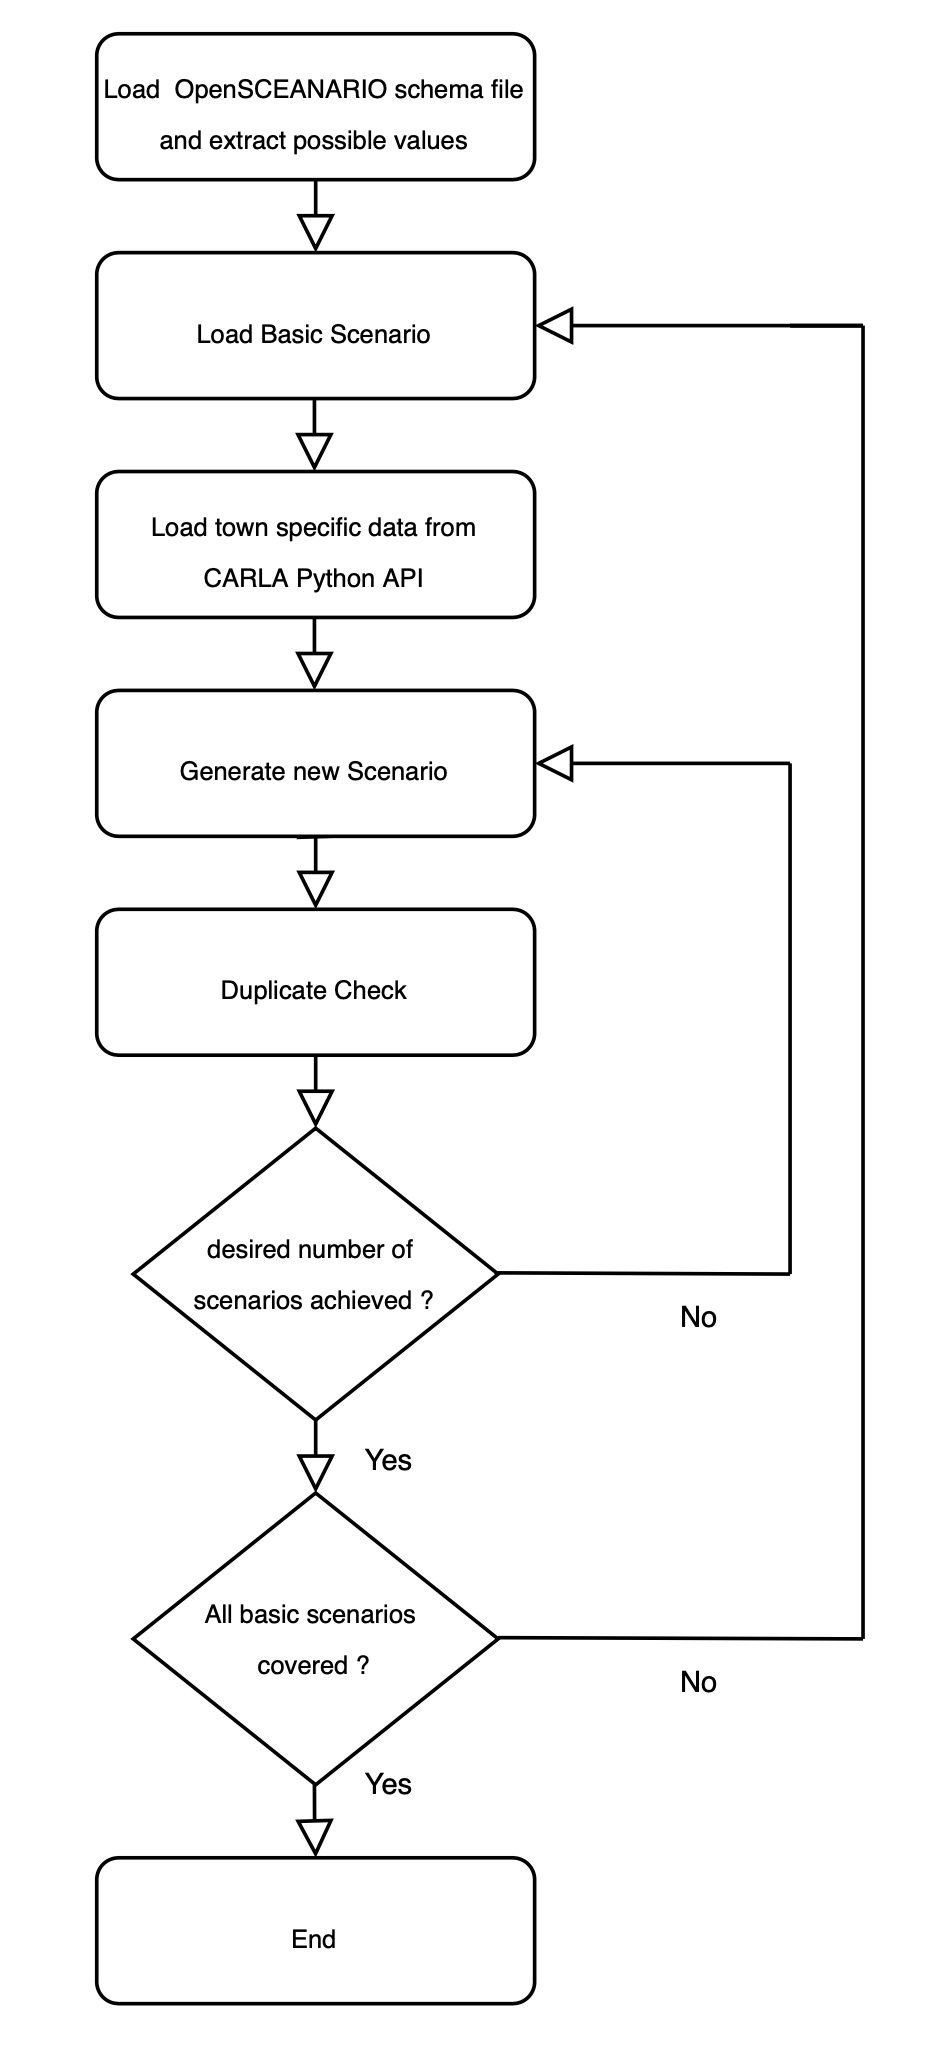
\includegraphics[width=0.9\linewidth]{figures/generator-flow.png}
	\caption{Flow-Chart of the scenario-generator.}
	\label{fig:generator-flowchart}
\end{figure}

\subsection{Adjustable parameters}

CARLA and the Scenario-Runner enable us to adjust quite a number of parameters, so that the generator can create a lot of diverse settings. In theory we have access to all possible parameters which contribute to a single scenario. Since most of them are interventions into the semantics of a scenario, we propose to first change parameters which do not change the overall actor behavior.
This includes the type and model of the car, which is steered by the agent, but more importantly of each and every other car.
This is important so that the model generalizes well, even if cars of different sizes, shapes and colors are in its field of view resulting in different RGB patterns perceived by the car's sensors.
Another parameter, that can be changed is the speed of the cars, which also has an impact on the behavior in critical situations.
This setting is not limited to cars and is used in a similar manner for bicycle and pedestrian types.

Moreover the weather plays an important role, as it drastically changes what is perceived by sensors and also alters the effects of certain behaviors. For example precipitation does not only impair the video of the camera, but additionally lengthens the breaking distance.
These variables can all be adjusted rather easily, by just randomly picking a value from the set of possible values.
Similar, we can adjust all available attributes for sun and fog tags.

In addition, we generate a random time of day for every new scenario to also cover an increasing danger in situations for example at night, where pedestrians and bicycles are harder to detect.

To also simulate a variety of different road conditions, we include a random generated friction scale factor for every new scenario. In real life, this could be influenced by many external effects for example oil spilled on the road.

However, these attributes are independent from the original spawn-position of all actors. 
The part of the configuration, which is more difficult to vary is with regards to further actors, such as pedestrians and other vehicles. These have to be spawned somewhere and a behavior needs to be defined.
CARLA provides a list of possible spawn points across a specific map, but if we just choose those randomly, we cannot be sure, that the spawned car has an impact on our scenario.
As an additional requirement, the generation of new scenarios should include a relocation of the scene to another suitable place in the same map or even to a different map.
At this time, we did not manage to extract a general process which is valid for all the basic scenarios. Therefore we had to do distinguish between the basic scenarios to transform every scenario to a different location or town by manually analyzing the situation.

For this, we first analyze the initial situation by fetching the closest town specific waypoints\footnote{CARLA provides waypoints, which are described as a 3D directed point including information about the location and orientation according to the lane. } based on the initial actor position. To get information about the scenario circumstances we use a simple approach to detect whether the scenario takes place at an intersection by calculating and comparing the distances between the actors and the hero (ego-vehicle) actor to the next intersection in driving direction. If the latter distance is less, we conclude that the scenario must take place at an intersection. This information is valuable for shifting the scenario to another  position in the same or different town. We do this with respect to all the conditions given by the initial scenario for instance by retaining the distances between all actors.
If we conclude that the scenario takes place at an intersection, we fetch all possible junctions using the Python API of CARLA for a specific map. The closest junction in driving direction based on the ego-vehicle position is used  as the scenario anchor. This anchor plays an important role in our concept of shifting a scenario to another place.

For some scenarios, it is typical that actor positions like for pedestrians or cyclists are not considered as waypoints since they spawn off-road.  If we detect such a deviation, we calculate an offset between the actual actor position and the nearest waypoint. To apply the correct orientation to a new position $p^{new}$, we rotate the offset using the position of the actor $p = (p_x,p_y,p_z)$ subtracted by the nearest waypoint $w = (w_x, w_y, w_z)$ with respect to the new orientation of the road $\Delta yaw = w_{yaw} - p^{new}_{yaw}$  using a rotation matrix with the difference in x direction $p_x - w_x$ and y direction $p_y - w_y$ indicated with $\Delta x$ and $\Delta y$ respectively:

\begin{equation}
	p_{new} = \left(\begin{matrix} cos(\Delta yaw) & sin(\Delta yaw) \\ - sin(\Delta yaw) & cos(\Delta yaw) \end{matrix}\right) *  \left(\begin{matrix} \Delta x \\ \Delta y \end{matrix}\right) 
\end{equation}


The considered distances and positions are illustrated  in Figure \ref{fig:distances_carla}, exemplary for the cyclist crossing scenario.

\begin{figure}[ht]
	\centering
	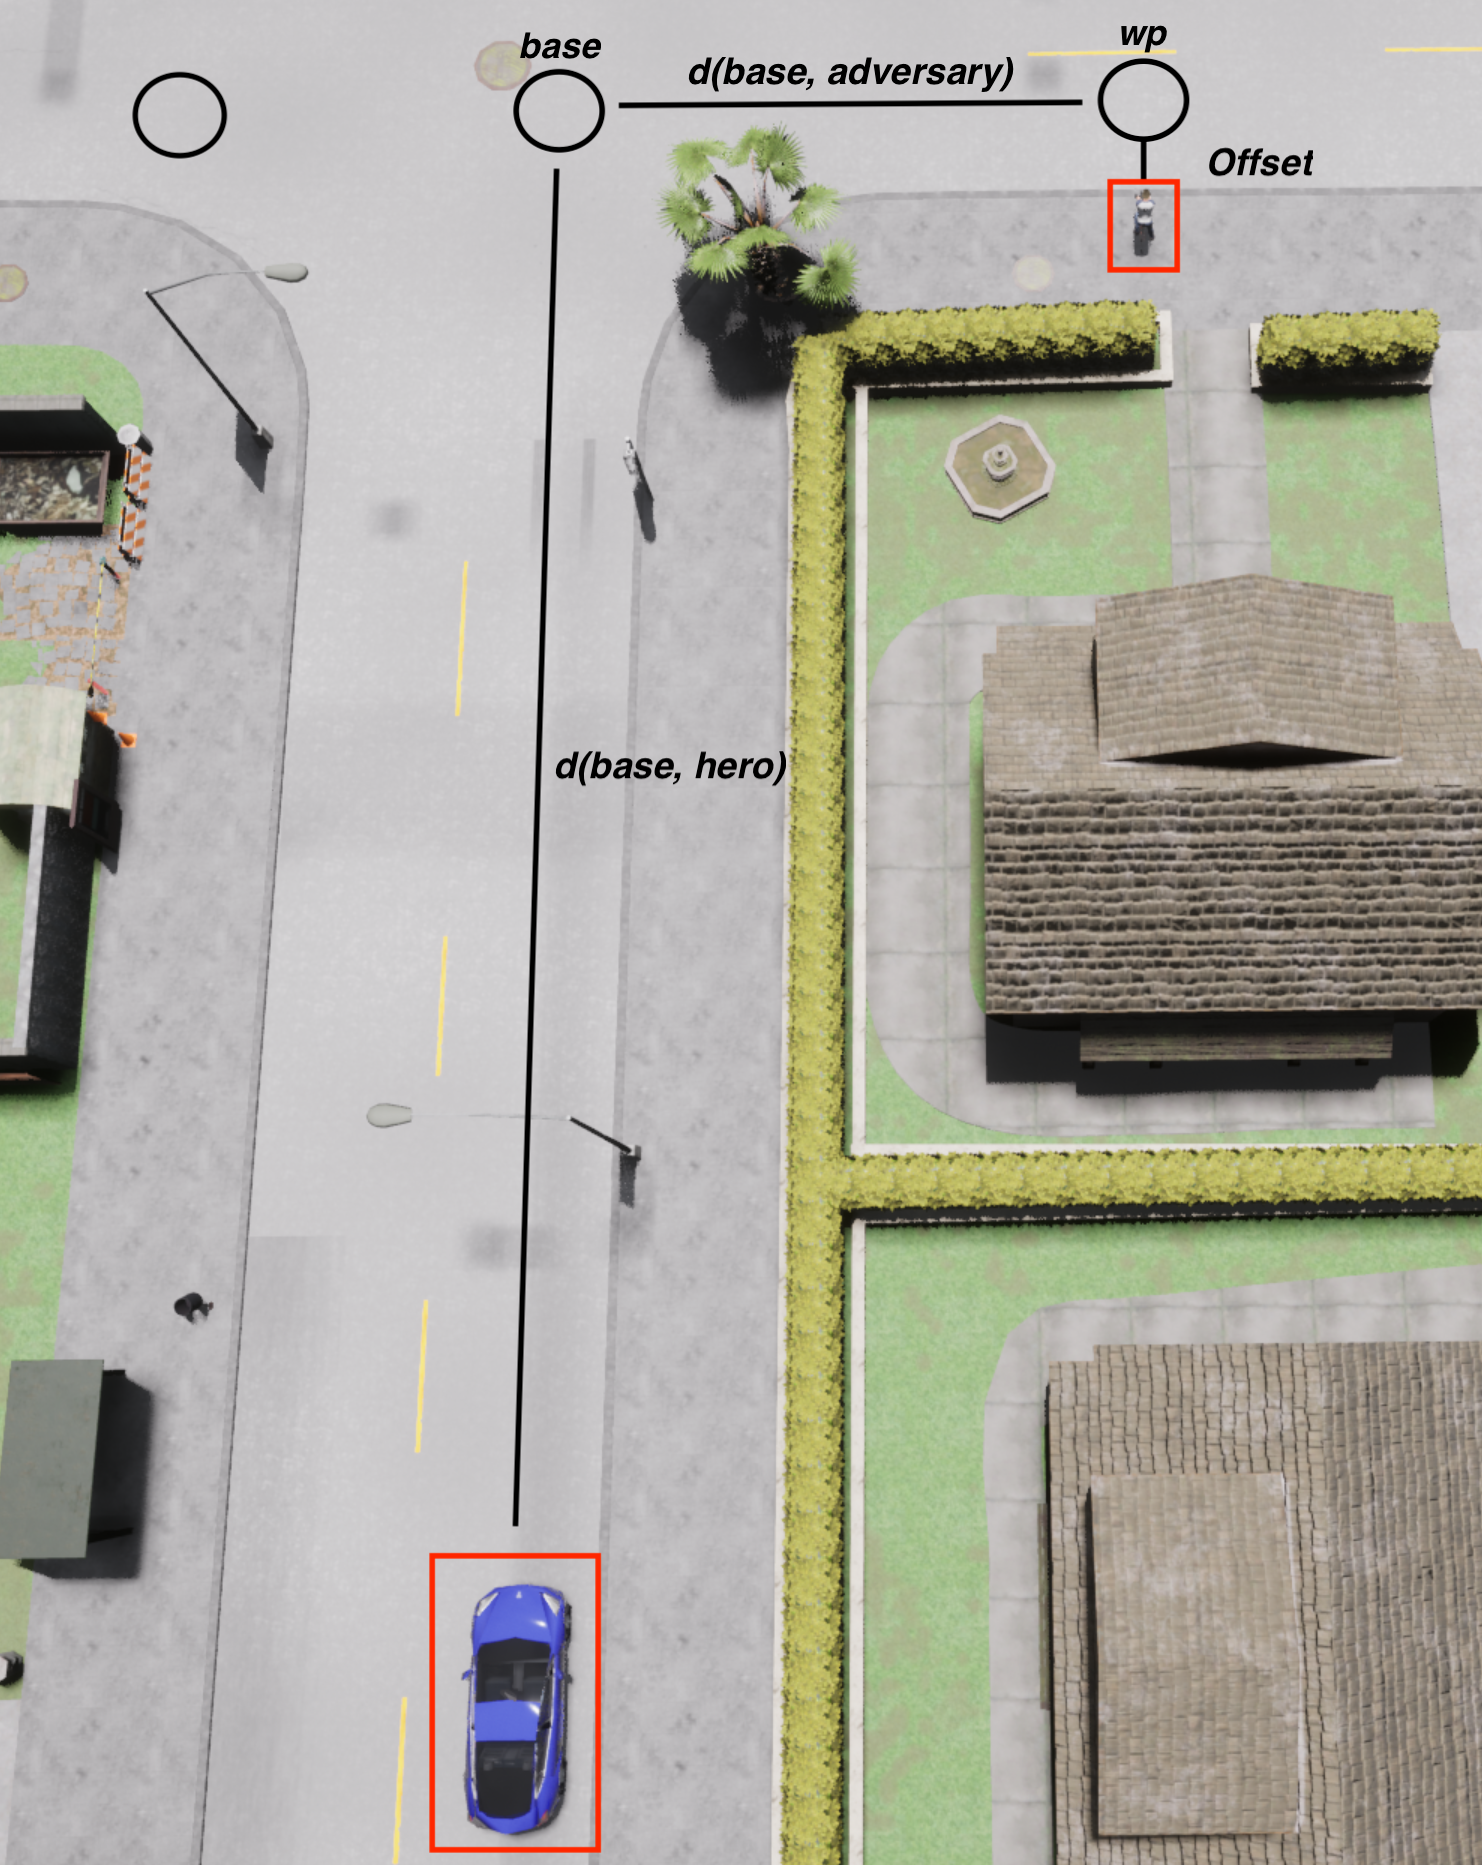
\includegraphics[width=\linewidth]{figures/carla_distances.png}
	\caption{Example of used distances and positions for transferring a critical cyclist crossing scenario to another intersection. }
	\label{fig:distances_carla}
\end{figure}

Not all positions calculated will work on different maps. Therefore we include different sanity checks when calculating new actor positions. In the example of the cyclist crossing scenario those checks include the validation of the car spawn point if the car's yaw is roughly the same as the junction's yaw and the spawn point of the cyclist  if the relation of the car and cyclist heading matches at the new waypoint.
To give an overview, \autoref{attribute_table} shows all parameters we declared as changeable for one new scenario. For every generator run, new values for the attributes will be set randomly.

\begin{table}
	\renewcommand{\arraystretch}{1.2}
	\caption{Changeable Attributes considered in the generator}
	\label{attribute_table}
	\centering
	\begin{tabularx}{\linewidth}{p{2cm}|p{2cm}|p{3.5cm}}
		\hline
		\bfseries Attribute & \bfseries Description & \bfseries Generation \\
		\hline\hline
		Road-Network/Map & Map where the scenario takes place & Random choice in a set of supported CARLA maps.  \\ \hline
		Vehicle color  & Color of the vehicle & Random RGB values. \\ \hline
		Vehicle name & Vehicle model type & Random choice from  a set of possible model types for a specific map. \\ \hline
		Pedestrian style & Pedestrian model type & Random choice from  a set of possible model types for a specific map. \\ \hline
		Pedestrian category & Pedestrian category & Random choice from a set of possible categories for pedestrians defined in the schema. \\ \hline
		Misc-Object Category & Category of a Misc-Object when available & Random choice from a set of possible categories for Misc-Objects defined in the schema. \\ \hline
		Actor position (including vehicles and pedestrians) & Initial spawn position of the vehicle & Random choice from suitable places fulfilling conditions of the initial scenario setup. \\ \hline
		Weather cloud state & Cloud state during the scenario & Random choice from a set of possible values defined in the schema. \\ \hline
		Fog visual range & Visual range for the driver & Random numeric value based on the initial value. \\ \hline
		Sun & Azimuth and intensity of the sun & Random numeric values based on the initial value. \\ \hline
		Precipitation & Precipitation type during the scenario & Random choice from a set of possible values defined in the schema. \\ \hline
		Dynamic constraints & Max acceleration, max speed and max deceleration of the vehicles  & Random numeric values based on the initial value. \\ \hline
		Time of day & Time of day the scenario starts play at & Random time between 0:00 am and 23:59pm. \\ \hline
	\end{tabularx}
\end{table}
\subsection{Limitations of scenario generation}
During our research, we found some limitations of the proposed approach for generating new scenarios. First, we experienced no determinism in the driving behavior and routing of the CARLA autopilot. Each map provided by CARLA has certain probabilities assigned for each situation where the driver agent has multiple routing options. Therefore it is not guaranteed that the autopilot will take the desired route. Using the cyclist crossing scenario as an example, the autopilot should make a right turn to trigger the scenario and therefore encounter a dangerous driving scene. But with the probabilities assigned, it could be the case that the autopilot turns left for a single run such that the scenario is not triggered or the driver is not confronted with the dangerous scene. Nevertheless, an agent could be used which is capable of following a specific route given by the scenario file.

Second, at this time it is not possible to gather semantic information namely concerning actor and driving behavior. In detail, the behavior of the base scenarios will be adapted without any behavior changes.  

The last limitation of our approach is the dependency to previously defined OpenSCENARIO basic scenarios. Since we use a predefined critical driving situation as a template, we are limited to currently six available scenarios. However, we think of OpenSCENARIO as a future-proof standard including a growing amount of available scenarios which can be used to create a variety of diverse scenarios.

\subsection{Imitation Learning Approach}
To test the generators' ability to generate diverse critical scenarios we can train a model on generated critical scenarios. We can then measure the performance of this model on a test set to see its robustness to newly generated scenarios. Using the existing functionality of the Scenario-Runner to play through our generated scenarios, we can gather the 'expert' driving data from the ego vehicle of the generated scenario. Using this data we are then able to train the vision agent.

The expert agent, which should be able to solve the critical scenario in the optimal way, uses information gleamed from the Carla Client. This includes precise weather readings, proximity measurements to other NPC actors and information pertaining the current traffic situation as well as details of other NPC actors' intentions and actions. This allows the expert to solve the scenario safely. The model to be trained however cannot be privy to any of this privileged information. Therefore the expert gathers data using an RGB camera sensor, mounted to the front of the ego car selected by the scenario generator. Multiple sensors such as side cameras or LIDAR were also available but to reduce the size of the collected data as well as the time required for training we opted into a single camera sensor. The only other data that was collected and provided to the model as part of its state vector was the steering, brake and throttle values.

The issue of the frequency of measurement is again a question of data volume and training time versus precision of the model as the frequency of data collection (dependent on resolution) could vary between 0-60 Hz depending on the hardware used. We opted for 5 collections per second with intent to vary this based on the effectiveness of the model trained on such sparse readings.

\section{Experiments}
\subsection{Imitation Learning Execution and Issues}
Though we set out to perform the learning as outlined in the approach we ran into some issues that prevented execution. 
First of all we started off by having a look at the approach as presented by \citeauthor{Xiao2020ActionBasedRL} in their work \citetitle{Xiao2020ActionBasedRL} \cite{Xiao2020ActionBasedRL, ActionBasedRL:github}. Although it looked promising and seemed straightforward, it turned out not to be executable at all.

So, we moved on and used \citetitle{felipecode:coiltraine} \cite{Toromanoff_2020_CVPR}. Using this framework we are able to train models based on image data and the experts control input. Additionally, this repository provides the functionality of validating a learned model as well as deploying a trained model in form of an agent and visualizing its behavior in the CARLA simulator.

After solving the problem of training a model, the next step was to collect the necessary data for training. For this purpose CARLA provides a data collector \cite{CARLA:DataCollector}, which works quite fine, but only with CARLA version 0.8.4. This is a major issue as the Scenario-Runner, which is used to execute our generated scenarios, only  offers support for CARLA versions 0.9 and higher. Due to this inconvenience we had to find our own way of recording all the necessary data for training a model.

We did so by modifying a Python script of the Scenario-Runner, namely \textit{manual\_control.py}. The functionality to record and save each frame of the camera attached to the car was basically already implemented. This only needed to be tweaked as such, that not every frame is saved, but it is limited to 5 fps and synced with the collection of the expert data. The expert data could be extracted by accessing CARLA via the Python API and we recreated how the CARLA data collector gathers this information. The data important for us (steering, throttle, brake) were collected rather easily, but when feeding this data to the training framework it apparently required more data.
Although we spent quite a lot of time with the framework and the data collection, we were not able to generate data such that COiLTRAiNE was able to learn a model.

Furthermore, even if we would have been able to provide the correct data, a lack of GPU hardware would have made the gathering of expert data an overwhelming task for our limited available resources, even at the low resolution of 200x300 we had seen in testing allowed for reasonable fps. This prevented any parallel data collection through a docker application or similar which caused gathering 500 MB of training data to take a minimum of 5 hours with 50 hours of driving time in the COiLTRAiNE training sets equating (albeit at a higher resolution) to roughly 50 hours of driving data.

Of course less data can be used, with 5 basic critical scenarios to be learned however and the span of possible changes in each one, which it is our aim to test, it is unrealistic to assume that 10 driving hours which our resources allowed us to gather would enable the model to achieve a level of competency. This assumption is based on the testing of pre-trained COiLTRAiNE sample models at a much higher resolution with 3 RGBA sensors accompanied by LIDAR data.

\begin{figure}[ht]
    \centering
    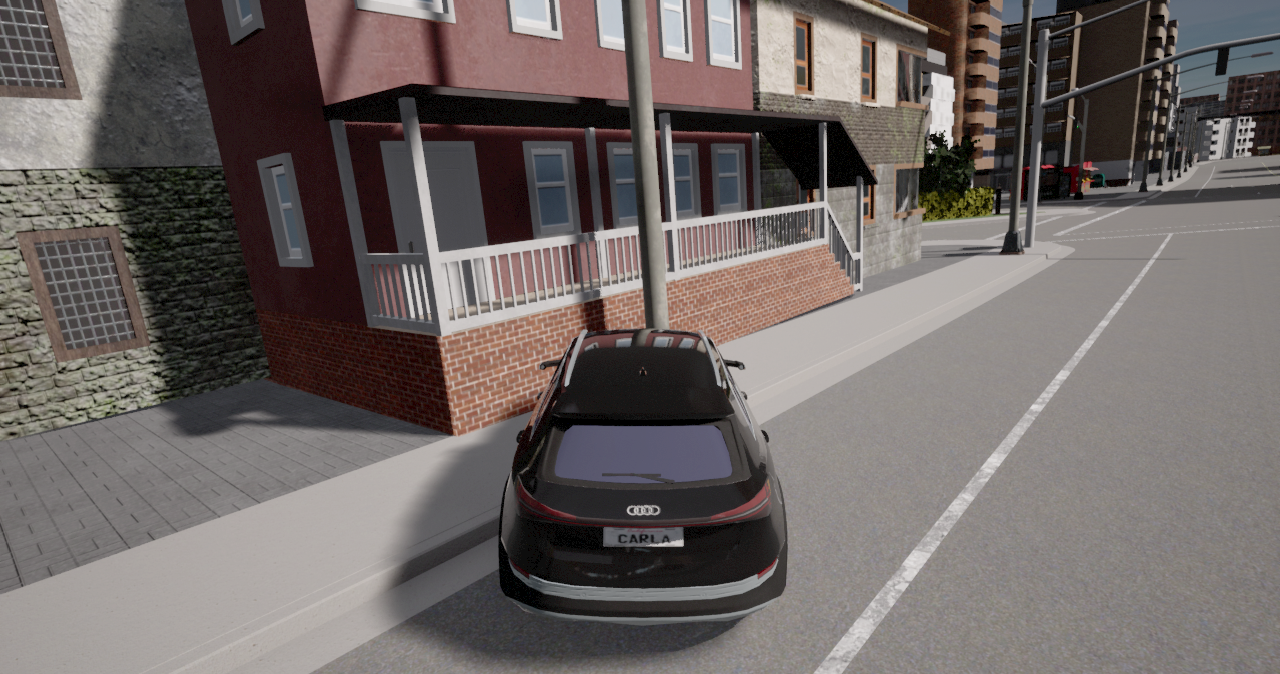
\includegraphics[width=0.9\linewidth]{figures/trained_agent_fail.png}
    \caption{Behavior of downloaded pre-trained model (in CARLA 0.9.9)}
    \label{fig:trained_agent_fail}
\end{figure}

Our last effort to validate the generated critical driving situations, was to observe an already learnt model from the paper \citetitle{Codevilla:OnOfflineEvaluation} \cite{Codevilla:OnOfflineEvaluation} and how it behaves in these scenarios. To do so we used the \textit{view\_model.py} from the COiLTRAiNE framework, which visualizes the model in the CARLA simulator. But although these models supposedly should behave quite well in most driving situations, there appeared to be some fundamental problems, as the agent could not even stay in its lane and on the street (as seen in \autoref{fig:trained_agent_fail}). The cause for this presumably lies in the different CARLA versions. The imitation learning framework was developed with version 0.8.4 in mind, but - in order for the Scenario-Runner to work - we had to use version 0.9 or higher.

\subsection{Imitation Learning takeaways}

Even though our experiments did not come to a positive end or enabled us to validate the generated critical scenarios by training a model, we learned quite a lot and want to share our key takeaways of the process.

First and foremost, the current situation regarding CARLA and its different versions is still subject to constant change. Especially with version 0.9 the whole Python API was changed. Therefore, it is quite dangerous to rely on frameworks developed for previous versions. This underlines that it was a good decision to choose the OpenScenario standard for the generated scenarios, as this will not be in danger to such change.
Due to the given timeframe a development of a learning framework from scratch in addition to the development of the generator for critical driving situations was just not viable.

Furthermore, we found out that it is possible to use the Scenario-Runner and a modified version of its manual control functionality to collect data. We even created a script to generate a bulk of critical scenarios and execute them via the Scenario-Runner to collect the data.
Although this consumes quite some time as the data is generated in real time, with enough resources and time at hand, this should not be a problem.

\section{Conclusion}
In this project paper we have presented a tool for generating new scenarios for the CARLA driving simulator. The focus of the scenarios was to represent critical driving scenarios since they are currently underrepresented in common datasets for autonomous driving challenges.
The proposed generator uses a predefined set of changeable attributes for defining a new scenario based on already present scenarios. After evaluating the possible methods supported by CARLA and its Scenario-Runner for defining new scenarios, we decided to use an approach utilizing the OpenSCENARIO standard. For this decision we considered generalization, number of adjustable parameters and simplicity. Our approach is able to generate new scenarios by changing static factors such as vehicle types, colors and weather as well as map specific factors such as spawn points or the map itself. The generator is able to create sufficiently different scenarios for every base scenario provided as OpenSCENARIO file (see \nameref{appendix} for some example generations). To ensure the novel scenarios are valid and diverse, the generator includes different sanity checks and a duplication check.

To evaluate the results of our scenario generator we initially planned to use imitation learning to train an autonomous driving model and validate whether it is robust against the critical scenarios. Although this was not possible due to a series of problems that occurred in the process, we were able to generate the essential data needed for imitation learning, i.e. the input of the camera sensor in form of images as well as the experts control input (throttle, brake, steering).

In future research, the generator could be enhanced by also supporting changes in the behavior of actors. This could lead to completely new scenarios. This requires a complete understanding of the abstract process on how actors behave also including the interaction of actors and a definition of a critical scenario such that only critical scenarios will be generated.
Future work could also consider including additional actors in the scenario by randomly spawning pedestrians or cars. For this, it should be ensured that those actors are only passively participating in the scenario to not interrupt the scenario flow.

The scenario generator should definitely be used as a solid basis for generating training data in future work. As the currently existing frameworks for imitation learning are not compatible with CARLA 0.9 and thus the Scenario-Runner, the development of such a framework working in unison with the scenario generator should be addressed in future work.
To conclude the work done for the scenario generator and the first research and approaches for using imitation learning to overcome the challenge of critical driving scenarios, we are quite satisfied with the results taking into account the issues and limitations we faced during this research.

\newpage
\printbibliography

\newpage
\onecolumn
\appendix\
\label{appendix}

\begin{figure}[h!]
    \centering
    \begin{subfigure}[c]{\textwidth}
        \centering
        \captionsetup{width=.9\linewidth}
        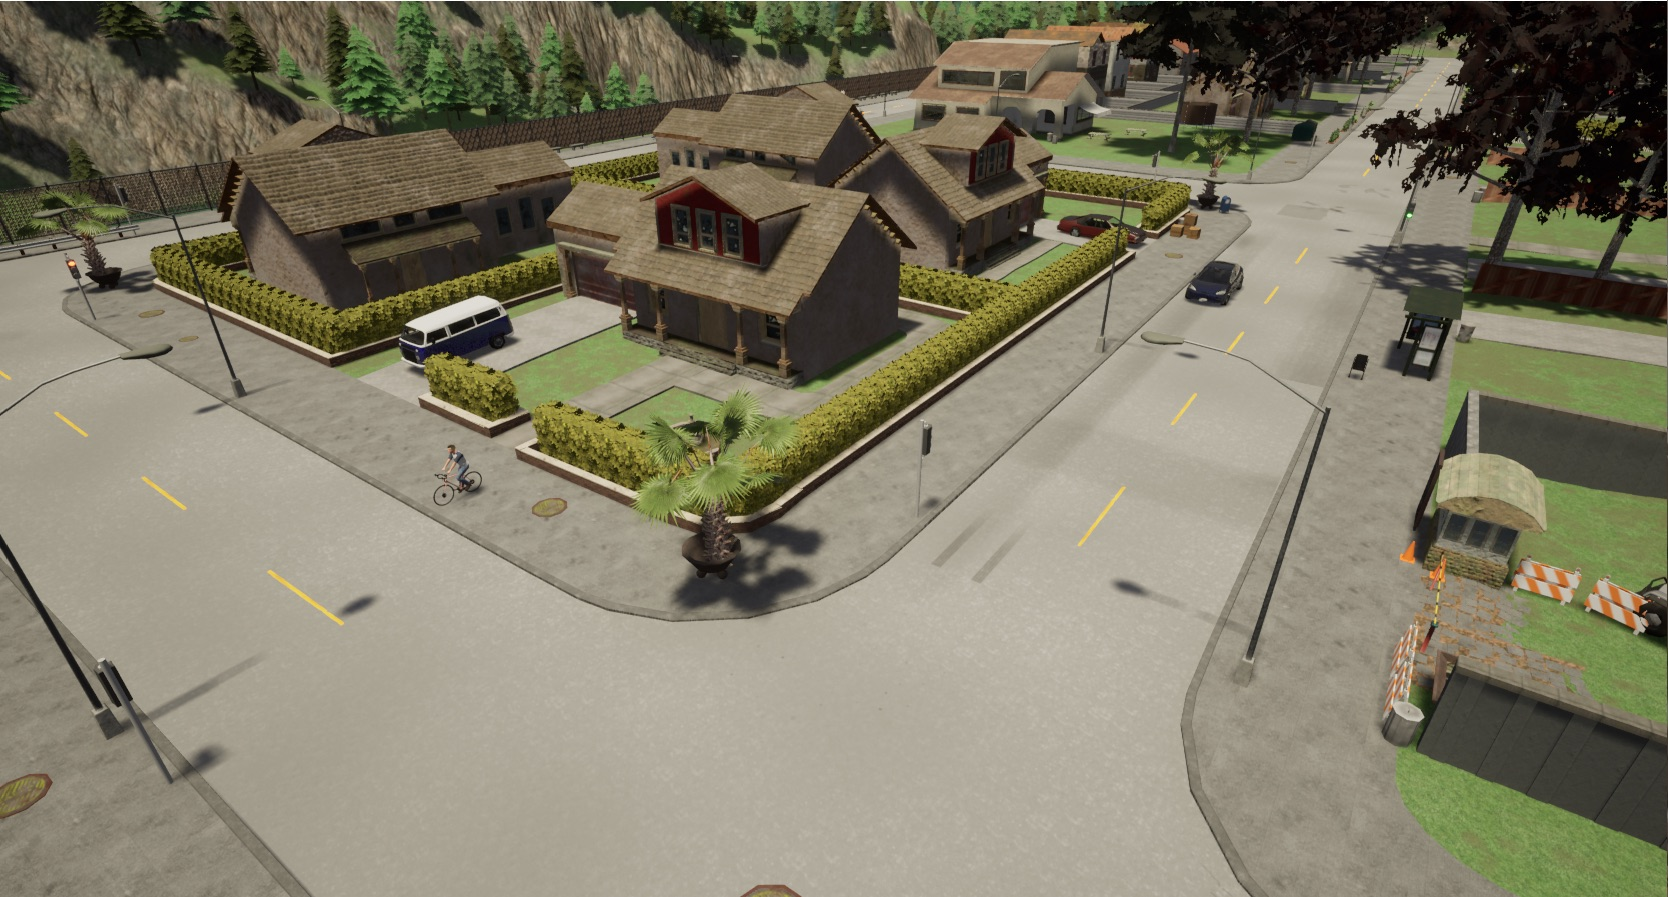
\includegraphics[width=0.6\textwidth]{figures/generated/cyclist_original.jpg}
        \subcaption{Original base scenario.} 
    \end{subfigure}
    \begin{subfigure}[c]{\textwidth}
    	\captionsetup{width=.6\linewidth}
        \centering
        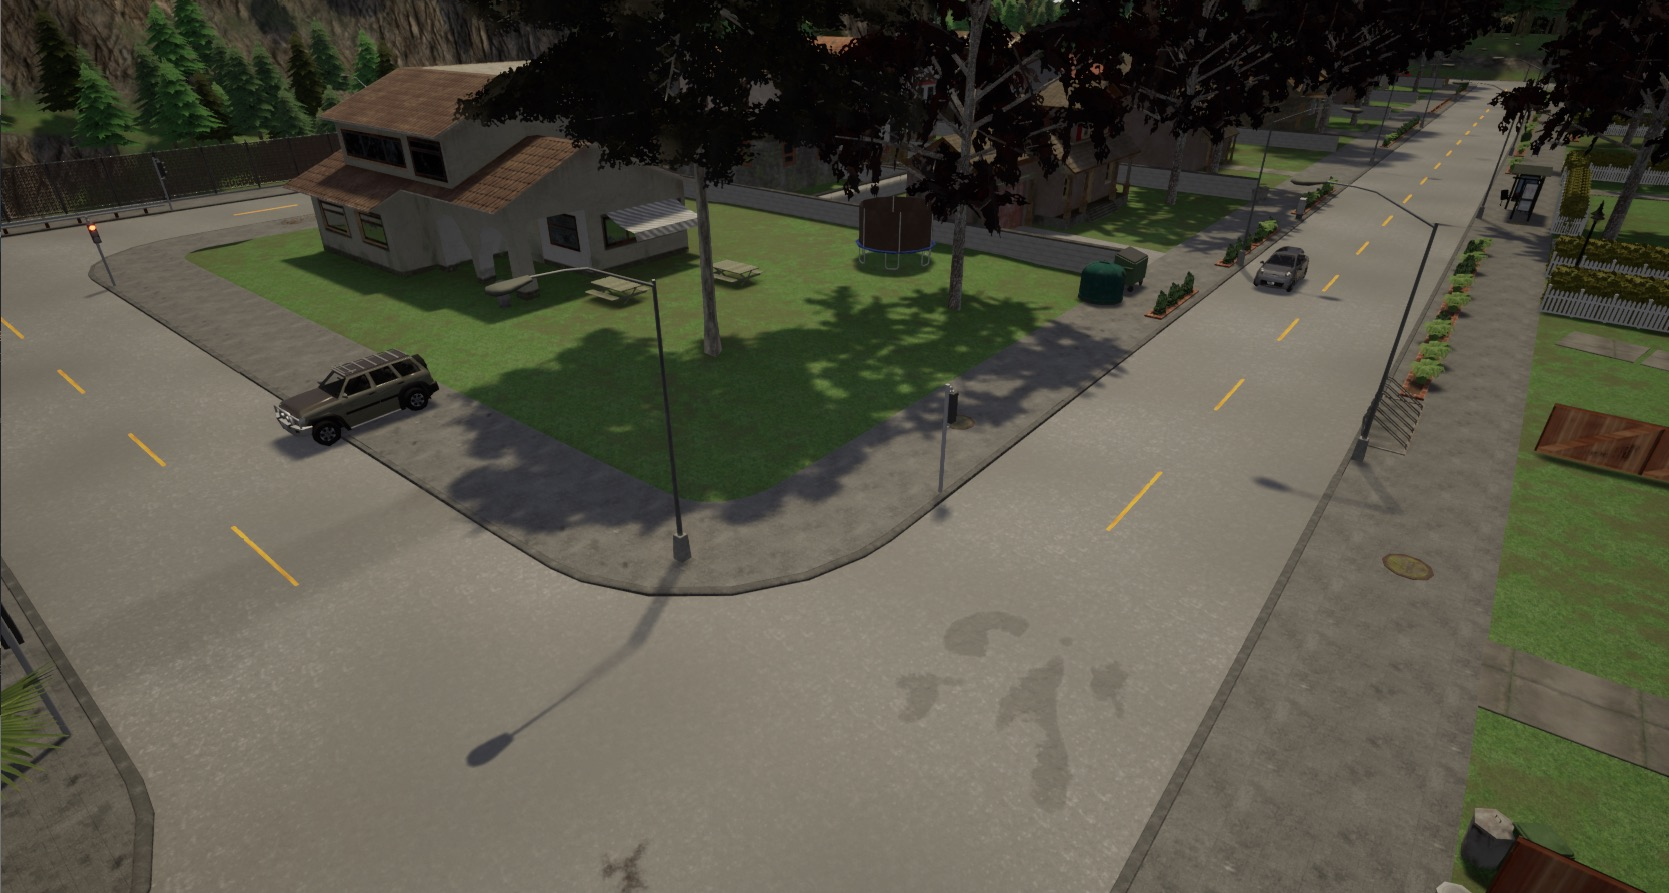
\includegraphics[width=0.6\textwidth]{figures/generated/cyclist_1.jpg}
        \subcaption{Example of a generated scenario in the same town as the original scenario but at a different intersection. (1)}
    \end{subfigure}
    \begin{subfigure}[c]{\textwidth}
    	\captionsetup{width=.6\linewidth}
        \centering
        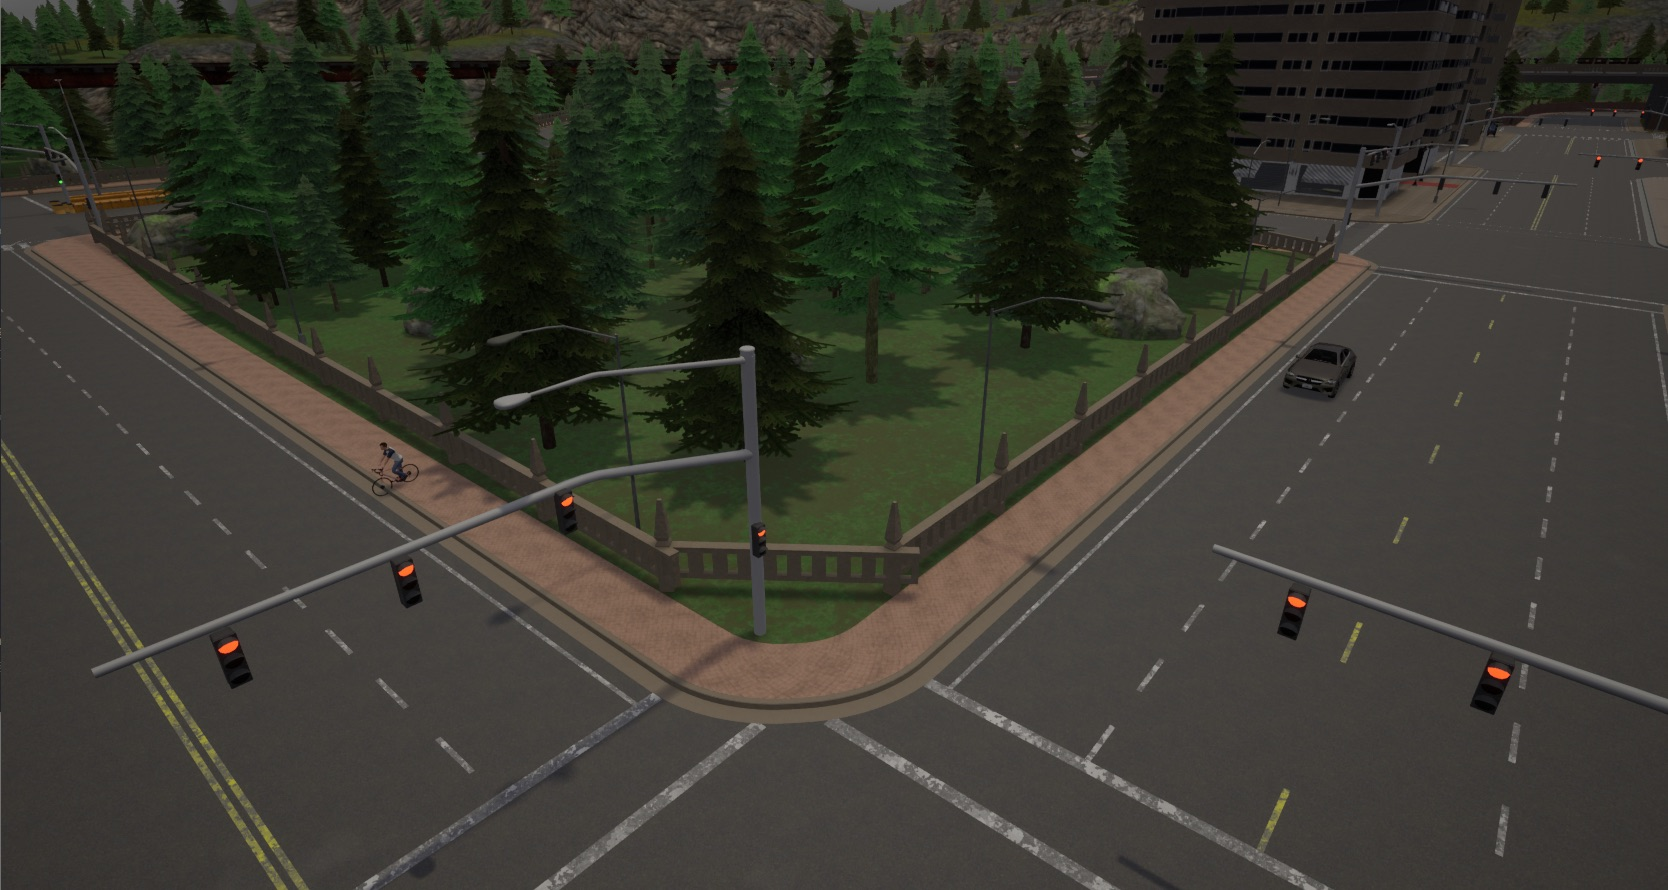
\includegraphics[width=0.6\textwidth]{figures/generated/cyclist_2.jpg}
        \subcaption{Example of a generated scenario in a different town but with the same scenario layout. (2)}
    \end{subfigure}
    \caption{Cyclist crossing scenario}
\end{figure}

\begin{figure}[h]
    \centering
    \begin{subfigure}[c]{\textwidth}
    	\captionsetup{width=.6\linewidth}
        \centering
        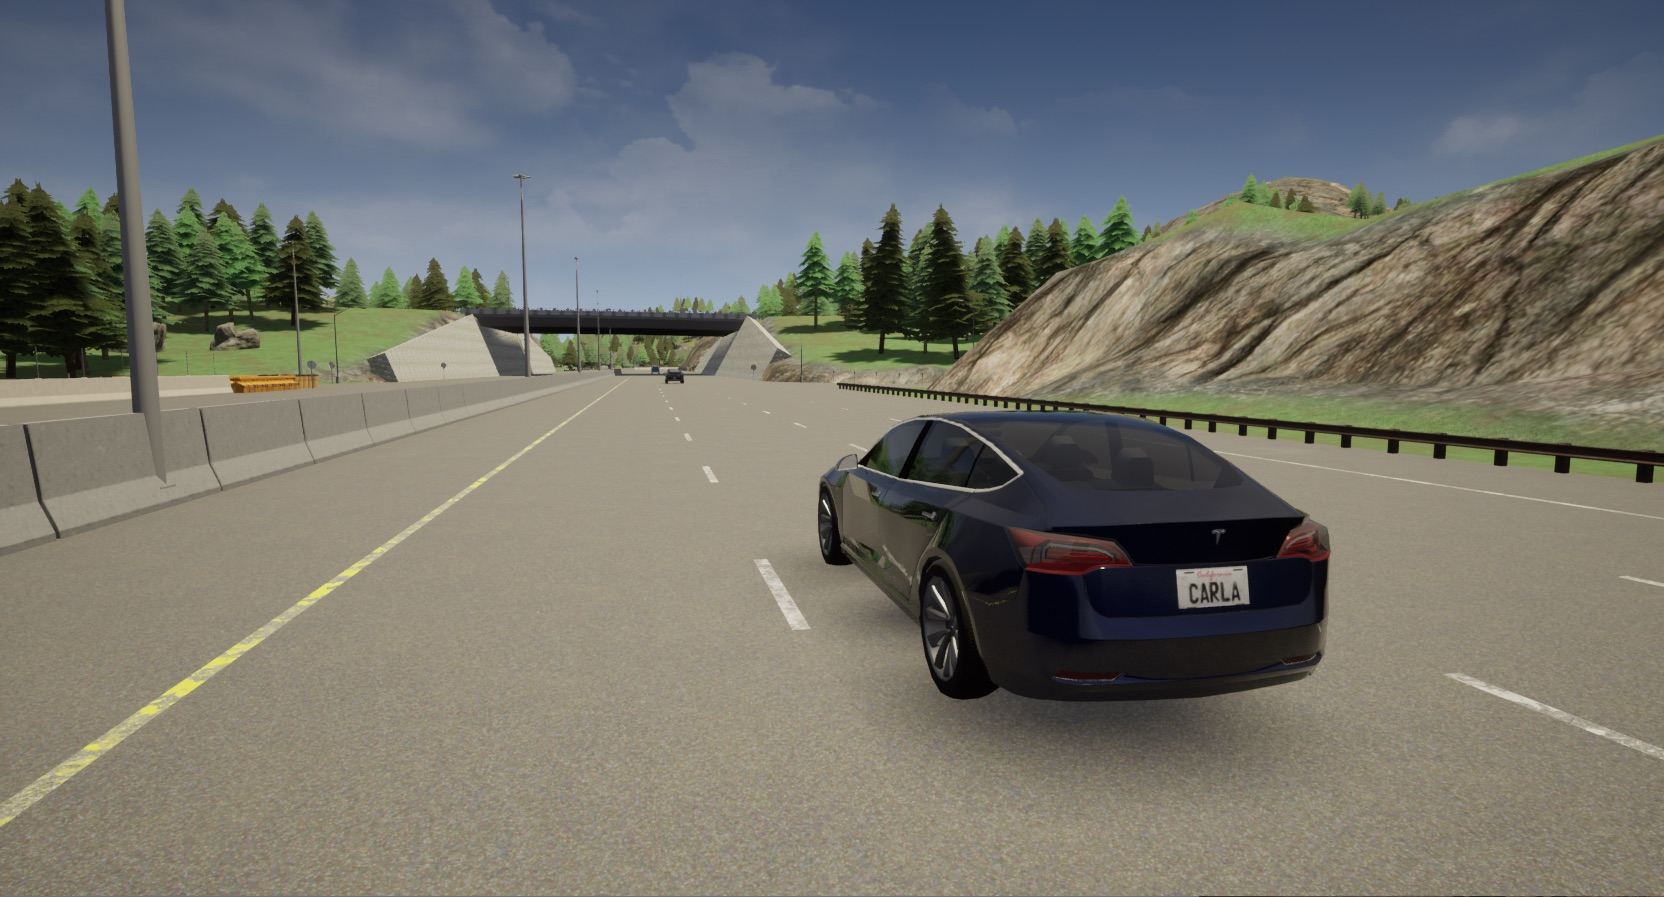
\includegraphics[width=0.6\textwidth]{figures/generated/lanechange_original.jpg}
        \subcaption{Original base scenario.} 
    \end{subfigure}
    \begin{subfigure}[c]{\textwidth}
    	\captionsetup{width=.6\linewidth}
        \centering
        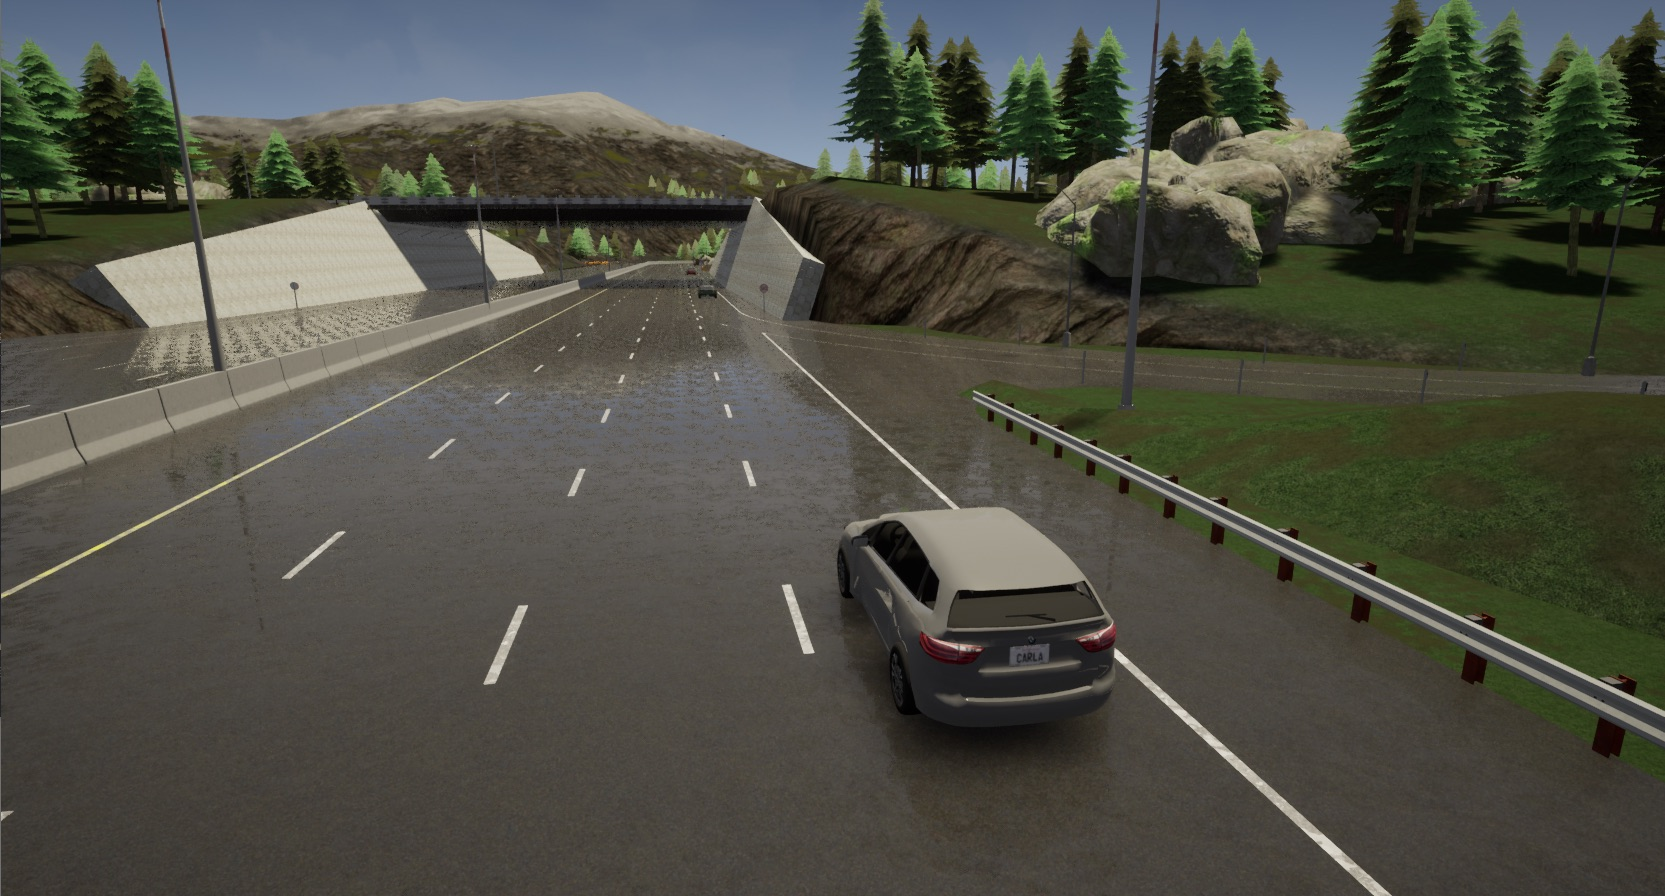
\includegraphics[width=0.6\textwidth]{figures/generated/lanechange_1.jpg}
        \subcaption{Example of a generated scenario in the same town as the original scenario. The vehicles have spawned in the opposite direction of the base scenario and use a different driving lane. (1)}
    \end{subfigure}
    \begin{subfigure}[c]{\textwidth}
    	\captionsetup{width=.6\linewidth}
        \centering
        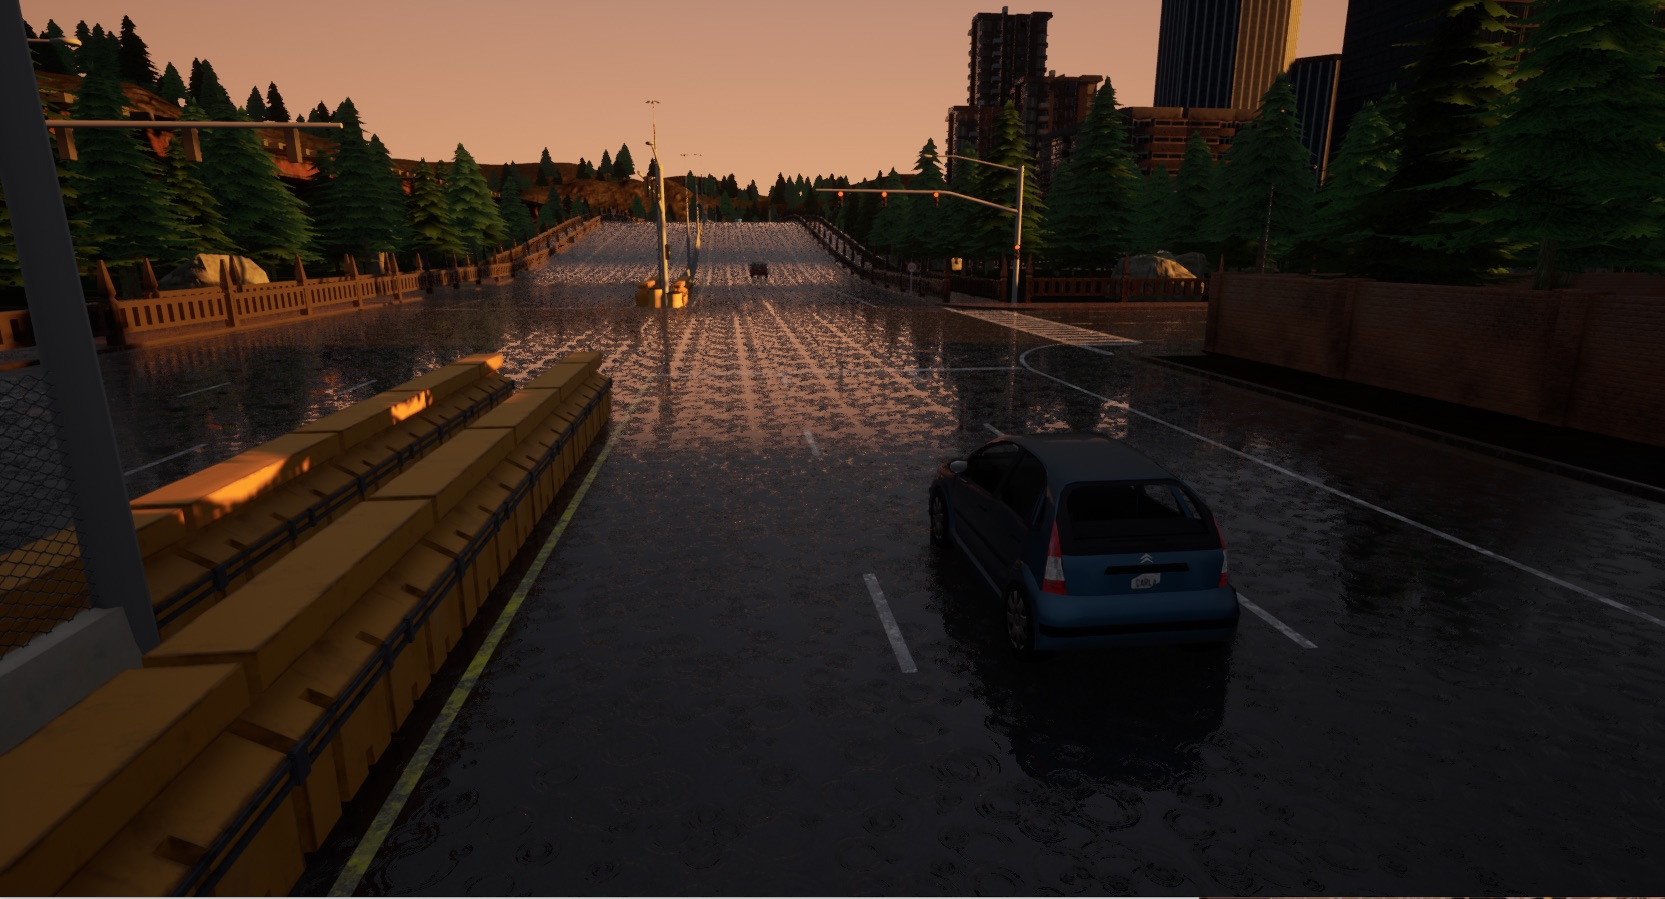
\includegraphics[width=0.6\textwidth]{figures/generated/lanechange_2.jpg}
        \subcaption{Example of a generated scenario in a different town. In the distance it can be seen that there is a slight incline in the road. (2)}
    \end{subfigure}
    \caption{Lane change scenario}
\end{figure}

\end{document}
